\chapter{Google App Engine.}\label{cap:GAE}
En este apartado de la memoria vamos a explicar lo que es, la configuración y como usar la plataforma Google App Engine.

\section{Introducción.}
Google App Engine es una conjunto de APIS que proporciona Google para construir tus propias aplicaciones web, que pueden ser alojadas y usadas en su servicio Google App y vendidas en Google Apps Marketplace. Además de alojamiento gratuito, Google ofrece un dominio, que es como el siguiente: \url{http://nombre\_de\_la\_aplicacion.appspot.com} y una base de datos propietaria de Google que se accede transparentemente a través de su API, gestión de usuarios mediante autentificación con cuentas Google del tipo: usuario@gmail.com, autentificación por federación o openID.

Además de todas estas características Google proporciona APIS para el desarrollo con Java, Python y Go, este último un lenguaje experimental propiedad de Google. Para usar dicha API, Google también proporciona un plugin para Eclipse, en caso de que el lenguaje elegido sea Java, que ayuda al despliegue de la aplicación web, auto completado y gestión de de las aplicaciones creadas. 

En el anexo~\ref{cap:configuracionGAEEclipse} se puede ver como instalar el plugin de Google App Engine para Eclipse.

En el proyecto se ha usado Java, por lo que las APIS de Python y Go no se han estudiado.

En general el uso de Google App Engine para desarrollar aplicaciones web es idéntico a crear una aplicación web con Java 2 Enterprise Edition (Java2EE), se pueden desarrollar servlet que recogen valores mediante métodos \lstinline{GET} o \lstinline{POST} y usar clases Java para hacer operaciones con ellos. A su vez para mostrar la información se pueden generar archivos *.jsp, que son archivos HTML con bloques o líneas de código Java incrustadas, que se introducen con estas etiquetas: \lstinline{<\%= linea de codigo Java \%>} o \lstinline{<\% bloque de codigo Java \%>}. A parte de archivos *.java y *.jsp, debemos tener una carpeta llamada war en la que tiene que ir toda la información de la aplicación web que queremos desplegar. En dicha carpeta hay varias subcarpetas como pueden ser css en la que tiene que ir el estilo de la web o WEB-INF en la que están todos los archivos de configuración, como pueden ser los permisos que tenemos que tener para poder acceder al uso de un servlet, si la web tiene conexión https, la configuración de la base de datos, etc. Más adelante se explicará con más detenimiento todas las carpetas de las que se compone un proyecto de Google App Engine.

Para este proyecto hemos tenido que desarrollar dos aplicaciones web, una que es un servidor de timestamp y otra que es una aplicación para gestión de las firmas digitales que realice cada usuario. A continuación vamos a explicar en profundidad la tecnología usada.

\section[Aplicación web genérica en GAE]{Explicación de una aplicación web genérica en Google App Engine.}
En esta parte voy a explicar en profundidad que es un servlet, los archivos de configuración, los archivos JSP y el resto de archivos necesarios para poder desplegar una aplicación en Google App Engine.
 
\subsection{¿Qué es un servlet?.}
Un servlet es la evolución de los antiguos applet de Java, su uso más común es generar páginas web dinámicamente con los parámetros que recibe mediante una petición realizada por el navegador web y datos que están almacenados en el servidor web.

Un servlet es un objeto Java que tiene que ser ejecutado en un servidor web o contenedor J2EE, que recibe unos parámetros, realiza una o varias acciones y devuelve un resultado que puede ser desde un código HTML, un JSP que genera dinámicamente un código HTML, un JSON o una simple cadena de texto.

Los servlets, junto con JSP, son la solución de Oracle a la generación de contenido dinámico equivalente al lenguaje PHP, ASP de Microsoft, Ruby, etc.

Los servlet forman parte de Java 2 Enterprise Edition (J2EE) que a su vez es una amplicación de Java 2 Standard Edition (J2SE), para su uso es necesario un servidor web que pueda interpretar código Java, el más famoso es Apache Tomcat que está desarrollado y mantenido por Apache Foundation, que son los encargados también de mantener y desarrollar el famoso servidor web Apache, aunque existen otro como JBoss, Jetty o GlassFish, pero como podremos ver no son los únicos, ya que el propio Google App Engine también funciona internamente a base de servlets y JSP.

Para crear un servlet hay que generar una clase Java que implemente la interfaz \lstinline{javax.servlet.Servlet} como puede ser \lstinline{javax.servlet.http.HttpServlet} que es un servlet específico para conexiones HTTP.
 
Una vez generada la clase hay que implementar el método \lstinline{doGet} para peticiones tipo \lstinline{GET} o el método \lstinline{doPost} para peticiones de tipo \lstinline{POST}. En el siguiente trozo se código se puede ver la implementación más básica de los métodos \lstinline{doGet} y \lstinline{doPost}.

\begin{lstlisting}[style=Java] 
@Override
protected void doGet(HttpServletRequest req, 
	HttpServletResponse resp) throws ServletException, IOException {
	// TODO Auto-generated method stub
	super.doGet(req, resp);
}

@Override
protected void doPost(HttpServletRequest req, 
HttpServletResponse resp) throws ServletException, IOException {
	// TODO Auto-generated method stub
	super.doPost(req, resp);
}
\end{lstlisting}

Una vez implementados los métodos que se necesiten se pueden usar el parámetro \lstinline{HttpServletRequest req} para recibir los valores que queramos enviar a la aplicación web y podemos usar \lstinline{HttpServletResponse resp} para enviar lo que queramos desde una redirección a un JSP, una página web, un JSON o una cadena de texto. 

Un ejemplo de como se reciben los parámetros sería: 

\begin{lstlisting}[style=Java]  
String num_sec = req.getParameter("sec");
\end{lstlisting}

Y si queremos devolver algo, por ejemplo un objeto \lstinline{JSONArray}:

\begin{lstlisting}[style=Java]   
PrintWriter out = resp.getWriter();
out.print(jsonArray);
out.flush();
\end{lstlisting}

Como podemos ver el objeto \lstinline{resp} nos da la posibilidad de conseguir un objeto \lstinline{java.io.PrintWriter} por el que podemos enviar lo que necesitemos.

La forma de acceder a un servlet mandándole peticiones \lstinline{GET} sería la siquiente: \url{https://servertimestamp.appspot.com/search?id=63&texto=Prueba}. Como podemos ver la dirección base es: \url{https://servertimestamp.appspot.com/}, el servlets estaría mapeado internamente en el servidor web, como ya veremos, en la dirección \url{/search} y el primer parámetro va precedido de \url{?id\_parametro} y el resto de \url{\&id\_parametro}. En nuestro ejemplo tendría dos parámetros que son \textit{id} y \textit{texto}, con sus valores después del =.

El método \lstinline{POST} es el utilizado para pasar parámetros por medio de formularios.

\subsection{¿Qué es JSP?.}
JSP es el acrónimo de JavaServer Pages y es una tecnología que ayuda a crear dinámicamente páginas web basadas en HTML o XML y es la solución equivalente a PHP de Oracle. En la figura~\ref{fig:modoJSP} podemos ver el proceso que se hace desde que se realiza la petición en el navegador hasta que se muestra un resultado.

\begin{figure}
  \centering
    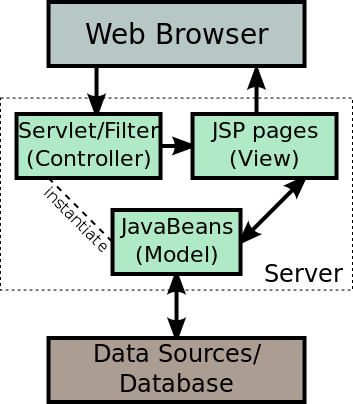
\includegraphics[scale=0.5]{./GoogleAppEngine/imagenes/JSP_Model.png}
  \caption{Modo de interpretación de un archivo JSP}
  \label{fig:modoJSP}
\end{figure}

Un fichero JSP es la unión de código HTML con código Java, el cual es interpretado en el momento de la visualización de la página web. Un ejemplo es el siguiente:
 
\begin{lstlisting}[style=HTML]   
<!DOCTYPE html>
<html>
<body>
<table>
<tr>
	<th>ID</th>
	<th>Num sec</th>
	<th>Token de tiempo</th>
	<th>Mensaje</th>
	<th>URL para ver la firma</th>
	<th>Fecha</th>
	<th>Usuario</th>
	<th id="filadestino">Destino</th>
	<th>Verificado?</th>
</tr>

<% for (RowRepositorioGeneral row : rows) {%>
<tr>
	<td><%=row.getId()%></td>
	<td><%= row.getNum_sec()%></td>
	<td><%=row.getToken_tiempo()%></td>
	<td><%=row.getTexto_claro()%></td>
	<td><a href=<%=row.getUrl_firma()%>>URL para ver el token
			de tiempo</a></td>
	<td><%=row.getFecha()%></td>
	<td><%=row.getUsuario()%></td>
	<td id="filadestino"><%=row.getDestino()%></td>
	<td>
		<%
		Boolean confirmado = row.getConfirmado();
		if (!(confirmado == null) && confirmado) {
		%>
		<center>
			<img src="ok.png" />
		</center> <%} else  %>
	</td>
</tr>
<%}%>
</table>
</body>
</html>
\end{lstlisting}

Como se puede ver en este trozo de código de este archivo JSP genera una tabla que se rellena dinámicamente con los valores que devuelve un objeto Java, se puede observar que se entrelazan trozos de código Java con etiquetas HTML. Si mostramos esta web y acto seguido introducimos otro objeto \lstinline{RowRepositorioGeneral} en la estructura, cuando recarguemos la tabla tendrá una fila nueva.

\subsection{La carpeta WAR.}

La carpeta WAR es la carpeta principal para el despliegue de una aplicación web, ya que en ella es donde se almacenan todos los archivos que se necesitan para el funcionamiento de la aplicación web, como pueden ser archivos HTML, CSS, JSP, imágenes, etc. En la figura~\ref{fig:carpetawar} se puede la carpeta WAR de una de las aplicaciones web realizadas.

\begin{figure}
  \centering
    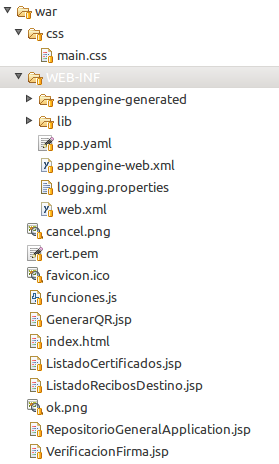
\includegraphics{./GoogleAppEngine/imagenes/carpetawar.png}
  \caption{Carpeta WAR}
  \label{fig:carpetawar}
\end{figure}

Se puede observar las diferentes carpetas y ficheros que la forman. Podemos ver que la carpeta css contiene los archivos de estilo que la página web usará, también podemos ver los archivos web.xml y app.yalm, que son archivos de configuración del servidor que se verán en el próximo apartado~\ref{cap:refArchivosConfiguracionGoogleAppEngine} y además los archivos JSP que se usan en la aplicación junto con los archivos HTML y JavaScript que se necesiten.

\subsection{Archivos de configuración.\label{cap:refArchivosConfiguracionGoogleAppEngine}}
Los principales archivos de configuración son web.xml y app.yalm, este segundo es solo una forma de escribir de forma más legible XML, para que nos sea más sencillo entenderlo.

Un ejemplo de un archivo web.xml es el siguiente:

\begin{lstlisting}[language=XML]
<?xml version="1.0" encoding="utf-8"?>
<web-app xmlns:xsi="http://www.w3.org/2001/XMLSchema-instance"
xmlns="http://java.sun.com/xml/ns/javaee"
xmlns:web="http://java.sun.com/xml/ns/javaee/web-app_2_5.xsd"
xsi:schemaLocation="http://java.sun.com/xml/ns/javaee
http://java.sun.com/xml/ns/javaee/web-app_2_5.xsd" version="2.5">

	<servlet>
		<servlet-name>AddRow</servlet-name>
		<servlet-class>pfc.ServletCreateRow</servlet-class>
	</servlet>
	<servlet-mapping>
		<servlet-name>AddRow</servlet-name>
		<url-pattern>/add</url-pattern>
	</servlet-mapping>

	<welcome-file-list>
		<welcome-file>ServerTimestampApplication.jsp</welcome-file>
	</welcome-file-list>
</web-app>
\end{lstlisting}

Como se puede observar en el código anterior se ha definido un servlet que se llamará \lstinline{AddRow} que usará la clase \lstinline{ServletCreateRow} y que estará mapeado en la dirección web \url{/add}, también podemos observar que el fichero que nos mostrará el servidor será \lstinline{ServerTimestampApplication.jsp} si entramos a la url principal.

A continuación podemos ver el aspecto de un archivo app.yalm:

\begin{lstlisting}[language=YAML]
application: repositoriorecibos
version: 1
runtime: java

handlers:
  - url: /add
    servlet: pfc.ServletCreateRow
    secure: always
welcome_files:
  - RepositorioGeneralApplication.jsp
\end{lstlisting}

Como podemos observar es mucho más fácil de entender y de escribir, el único problema que tienen los archivos YALM es que son sensibles a los espacios en blanco y tabulaciones, por lo que hay que tener cuidado a la hora de redactarlos. En este archivo se crea un servlet en la ruta \url{/add}, que es la clase Java \lstinline{ServletCreateRow} del paquete \lstinline{pfc} y que siempre hay que estar registrado en la aplicación para poder acceder a él. También podemos observar el fichero de bienvenida para cuando accedemos a la aplicación web. 

Al tener el archivo app.yalm en la carpeta WEB-INF el parseador de YALM  interpreta dicho archivo y genera automáticamente un archivo web.xml que usará el servidor web para su configuración.

Para ver todas las opciones de configuración que se pueden modificar en app.yalm o en web.xml se puede consultar los siguientes enlaces \url{https://developers.google.com/appengine/docs/java/config/} y \url{https://developers.google.com/appengine/docs/java/configyaml/}. En el primero podemos ver todas las opciones configurables de web.xml y en el segundo las de app.yalm.


%%----------------------------------------------
%% Hasta aquí diseño, el resto es implementación
%%----------------------------------------------


\section{Servidor de timestamp.}

En este apartado vamos a explicar en profundidad todo lo relacionado con la aplicación de timestamp que he tenido que desarrollar, desde el diseño que se ha seguido hasta los problemas que me han surgido.

En principio me gustaría explicar para que se usa un servidor de timestamp en general. Un servidor de timestamp es un registro donde cualquier persona puede subir un documento y el servidor guarda ese documento añadiéndole la fecha en la que se realizó la subida, dicha aplicación luego ofrece el servicio de consultar a que hora fue subido dicho documento. Un ejemplo podría ser \url{https://seguro.ips.es/servidortimestamp/index.asp} que se puede ver una captura de pantalla en la figura~\ref{fig:server_ips_timestamp}. En dicha captura podemos ver que tiene las opciones básicas de un servidor de timestamping como puede ser generar un sello, consultar su validez, etc. 

\begin{figure}[h]
  \centering
    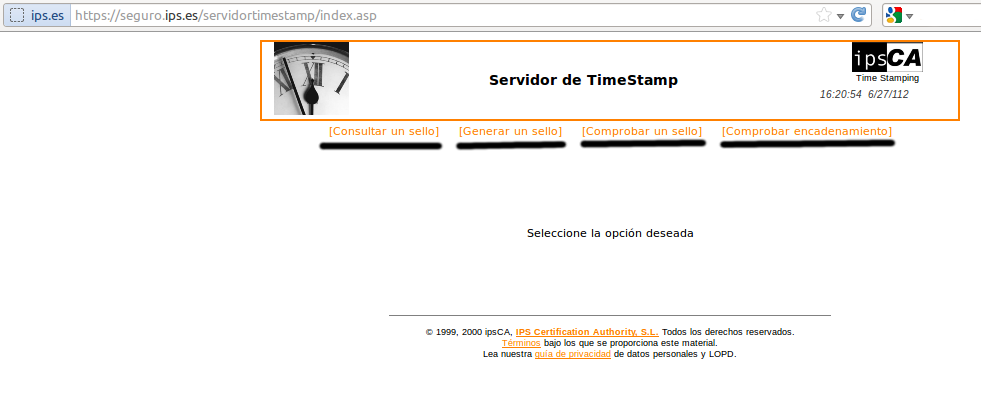
\includegraphics[scale=0.5]{./GoogleAppEngine/imagenes/server_ips_timestamp.png}
  \caption{Servidor Timestamp https://seguro.ips.es/servidortimestamp}
  \label{fig:server_ips_timestamp}
\end{figure}

La veracidad de que el sellado de dicho documento fue en el instante que dice ser, depende de la confianza que se tenga en ese servicio. Es similar a cuando se necesita que te sellen un documento físico, que dependiendo de quien lo necesite, necesitamos que lo firme un notario, un empleado público, etc. Normalmente suelen existir servidores de timestamping en los que se tiene confianza y los documentos sellados se consideran verdaderos.

Existen tres modelos principales de servidor de timestamping que son los siguientes:

\begin{itemize}

\item \textbf{Solución Arbitrada básica:} En esta solución el usuario que quiere sellar algo mandaría una copia del documento que quiere sellar a la entidad de sellado, que pondría el sello de tiempo y guardaría una copia de dicho documento, este es el modelo más parecido a la vida real. Esta solución tiene un par de grandes problemas como puede ser la privacidad del documento que se pierde totalmente, tenemos que tener en cuenta que el servidor de timestamping puede estar en España, EEUU o en cualquier otro país y a su vez la base de datos para almacenar todos los documentos tendría que ser enorme, por lo que almacenar todos los documentos nos puede acarrear muchos problemas.

\item \textbf{Solución Arbitrada avanzada:} Esta solución es una evolución de la anterior, en ella el cambio que se hace es que el usuario que quiere que le sellen el documento manda el hash de dicho documento y la entidad solo tendría que almacenar dicho hash junto con el sello de tiempo que se ha generado. Esta solución no tiene los inconvenientes de la anterior, ya que el tamaño de los documentos se reduciría a unos pocos bytes y la privacidad del documento no se ve comprometida. El problema que si persiste es que el usuario conozca a la entidad de certificación y puedan generar timestamp falsos, pero este problema depende de la confianza que queramos darle a ese servicio, supondremos que si es un servicio oficial y serio este problema no va a ocurrir, de todas formas existen otras soluciones que arreglan dicho problema.

\item \textbf{Solución Arbitrada avanzada y distribuida:} Esta forma consigue arreglar el problema de la anterior que se produzca un uso fraudulento del servidor de timestamping. La solución es usar varias entidades de timestamping, por lo que el usuario mandaría el hash a varias entidades de sellado y guardaría los reguardos que están firmados digitalmente de todas las entidades. Así si en una hay un problema tendría varias replicas de que la firma se realizó en ese momento en concreto.

\item \textbf{Solución mediante enlaces:} Esta solución es la más compleja y a su vez la que soluciona todos los problemas anteriores, además tiene la ventaja de que no tiene que usar multitud de entidades de certificación. Consiste en que cuando un usuario quiera sellar un documento, mande el hash del documento, la entidad añade el número de serie del documento anterior, el timestamp y lo firma digitalmente, por lo que el problema de que se introduzcan valores fraudulentos por mitad se anula, ya que cada recibo está enlazado con el anterior.
\end{itemize}

En nuestro caso hemos desarrollado un servidor de timestamping en su versión solución arbitrada avanzada.


\subsection{Explicación de la aplicación web.}
%TODO: falta explicar como funciona la BD...
En este capítulo vamos a explicar todas las partes que componen la aplicación web que hemos desarrollado para la implementación del servidor timestamp.

En la figura~\ref{fig:paquete_pfc} se puede ver las clases que forman el paquete \textit{pfc}.

\begin{figure}
  \centering
    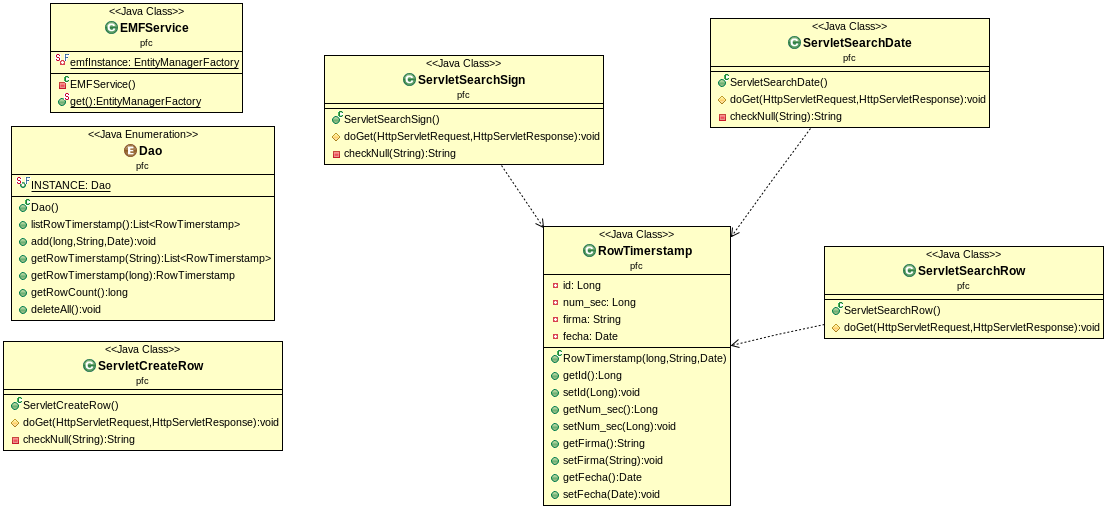
\includegraphics[scale=0.6]{./GoogleAppEngine/imagenes/UML_pfc.png}
  \caption{Detalles del paquete pfc}
  \label{fig:paquete_pfc}
\end{figure}

A continuación vamos a explicar una por una las clases desarrolladas para el funcionamiento del servidor de timestamp.

\begin{itemize}

\item \textbf{Dao.java:} esta clase es la encargada de todos los accesos a la base de datos, desde la inserción, el borrado y el listado de las filas, hasta consultas que se necesiten. Se puede ver que las sentencias que son listado de columnas se realizan con una sentencia SQL, se puede ver un ejemplo es el siguiente trozo de código:

\begin{lstlisting}[style=Java]
EntityManager em = EMFService.get().createEntityManager();
Query q = em.createQuery("select t from RowTimerstamp t where t.num_sec = :num_sec");
q.setParameter("num_sec", id);
RowTimerstamp RowTimerstamps = (RowTimerstamp)q.getSingleResult();
\end{lstlisting}

Pero las consultas que implican inclusión o borrado de filas no se realizan mediante sentencias SQL convencionales, se realizan con métodos que proporciona la API, un ejemplo es el siguiente trozo de código:

\begin{lstlisting}[style=Java]
EntityManager em = EMFService.get().createEntityManager();
RowTimerstamp RowTimerstamp = new RowTimerstamp(num_sec, firma, fecha);
em.persist(RowTimerstamp);
em.close();
\end{lstlisting}

\item \textbf{RowTimerstamp.java:} en esta clase se diseña el formato de las filas de la base de datos, que como se ha explicado anteriormente no se crea con sentencias SQL, se usa un modelo de programación llamado JPA. Para dicho modelo hay que crear una clase que contenga como variables de clase, las columnas que formarán la tabla en la base de datos. Como podemos ver, mediante un mecanismo llamado anotaciones Java, se le indica si el campo es la clave primaría, si es auto incrementado y otras opciones que habría que indicar en la creación de la tabla. A continuación podemos ver un trozo de código con las variables que posteriormente serán las filas de la tabla que queremos crear.  

\begin{lstlisting}[style=Java]
@Id
@GeneratedValue(strategy = GenerationType.SEQUENCE)
private Long id;
private Long num_sec;
private String firma;
private Date fecha;
\end{lstlisting}

Se puede ver que el campo \lstinline{id} será la clave primaría, que se indica mediante la anotación \lstinline{@Id} y que será auto incremental, a su vez también podemos ver el resto de datos que se van a almacenar, el campo \lstinline{num_sec} que es el número de secuencia, ya que el campo \lstinline{id} lo usa la base de datos para organizarse internamente, el campo \lstinline{firma} que es hash firmado por el usuario, el campo \lstinline{fecha} como su nombre indica es la fecha en la que se subió el hash firmado. El resto de métodos que tiene esta clase son un constructor, getter para consultar los campos y setter para insertar valores.

\item \textbf{ServletCreateRow.java:} esta clase es un servet que se encarga de recibir todos los parámetros necesarios y añadirlos a la base de datos. Al recibir los parámetros mediante \lstinline{GET} tiene que implementar el método \lstinline{doGet}, casi todos los servlets implementados en el proyecto mandan los parámetros mediante \lstinline{GET}. La forma de recibir parámetros es la siguiente:

\begin{lstlisting}[style=Java]
String firma = req.getParameter("firma");
\end{lstlisting}

El resto de parámetros que se necesitan se generan en el servidor para que no puedan ser falseados, como es el número de secuencia y la fecha. Si la inserción se produce correctamente se devuelve una cadena que tiene el siguiente formato: ``ok;;num\_sec;;fecha", que será interpretado en la aplicación móvil y parseará dicha cadena para conseguir los valores que necesitemos.

%Quitado porque se pueden borrar datos que queramos con el dashboard
%\item \textbf{ServletDeleteAll.java:} es un servlet ``secreto" que se usa para borrar todas las filas del servidor, cosa que no se debería poder para no poder falsear los datos introducidos en el servidor de timestamp. Hay que llamarlo con un parámetro que es \textbf{borrar} con valor \textbf{5}.

\item \textbf{ServletSearchDate.java:} es un servlet que devuelve una cadena con la fecha de una fila que tiene el número de secuencia que se le pasa en el parámetro \lstinline{token}.

\item \textbf{ServletSearchRow.java:} es un servlet que devuelve una página web donde se puede observar en una única fila con toda la información almacenada correspondiente al número de secuencia que se le pasa mediante el parámetro \lstinline{id}. A continuación se puede ver un trozo de código que lo realiza:

\begin{lstlisting}[style=Java]
PrintWriter pw = resp.getWriter();
pw.print("<!DOCTYPE html>");
pw.print("<html><head><title>Lista Time Stamp</title><link rel=\"stylesheet\" type=\"text/css\" " + "href=\"css/main.css\"/> <meta charset=\"utf-8\"> </head>");
pw.print("<body><table><tr><th>ID</th><th>Num sec</th><th>Firma</th><th>Date</th></tr><tr> " + "<td>"+ row.getId() +"</td><td>"+ row.getNum_sec() +"</td><td>"+ row.getFirma() +"</td><td>" +	row.getFecha() + "</td></tr> </table></body>");
pw.flush();
\end{lstlisting}

Como se puede ver se crea una tabla en una web, con la etiqueta \lstinline{<TABLE>} y su fila se rellena dinámicamente dependiendo del número de secuencia que se le pase como parámetro.

\item \textbf{ServletSearchSign.java:} Es un servlet que devuelve una cadena con la firma que corresponde al número de secuencia que se pasa por el parámetro \lstinline{token}.

\end{itemize}

La mayoría de estos servlet son usados por la otra aplicación web o por la aplicación móvil para realizar comprobaciones o mostrar información.

%TODO: falta los jsp

\section{Servidor de registro de firmas.}

El servidor de registro de firmas que hemos desarrollado es una aplicación web en la que los usuarios pueden consultar las firmas realizadas, las firmas de las que es destino, gestionar sus certificados de clave pública, verificar una firma realizada por otro usuario, exportar una cadena con la que cualquier usuario pueda consultar si la firma que has realizado es válida, que se usará en comprobaciones en caso de que ocurra algún problema y generar códigos QR para que que otros usuarios puedan firmarlo.

El sistema de gestión de usuarios lo proporciona Google y para entrar en la aplicación web hay que poseer una cuenta de Google Account, si no se está logueado se produce una redirección a la página de logueo, que la podemos ver en la figura~\ref{fig:logueoRepoGeneral}. La parte de la seguridad de los usuarios, logueo y mantenimiento de las base de datos lo realiza Google.

\begin{figure}[h]
  \centering
    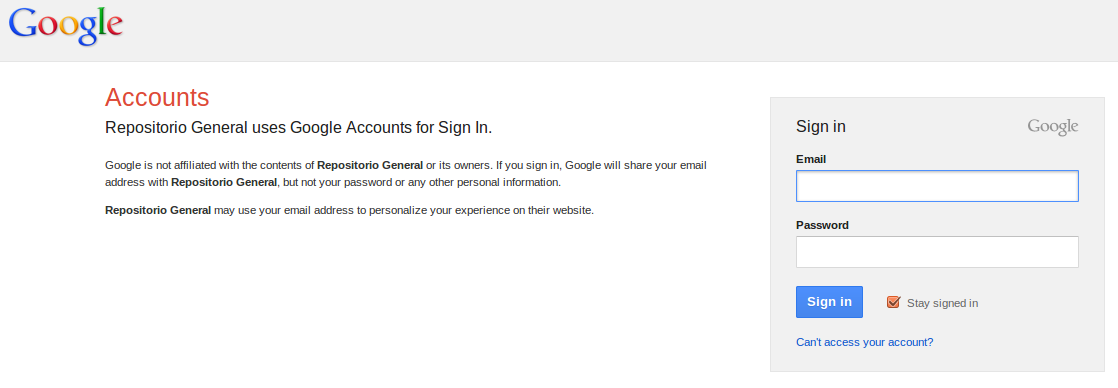
\includegraphics[scale=0.5]{./GoogleAppEngine/imagenes/login_repositorio_general.png}
  \caption{Login en Repositorio General}
  \label{fig:logueoRepoGeneral}
\end{figure}

La aplicación web se puede ver en la figura~\ref{fig:repositorio_general}, podemos ver que tiene varias pestañas, que se explicarán posteriormente, pero principalmente cada una de ellas se encarga de realizar una de las funciones que hemos comentado antes.

\begin{figure}[h]
  \centering
    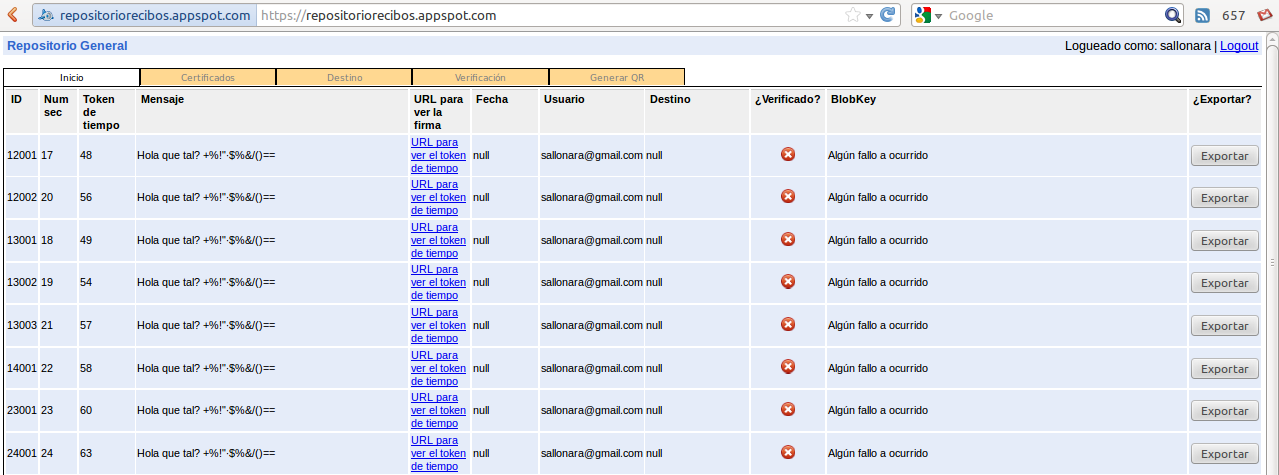
\includegraphics[scale=0.4]{./GoogleAppEngine/imagenes/repositorio_general.png}
  \caption{Repositorio General}
  \label{fig:repositorio_general}
\end{figure}

\subsection{Explicación de la aplicación web.}

%TODO: falta explicar como funciona la BD...
En la figura~\ref{fig:clasesReposotorioGeneral} se puede ver las clases que forman el paquete \textit{pfc} de la aplicación web repositorio general. A continuación vamos a explicar una por una las clases desarrolladas.

\begin{figure}[h]
  \centering
    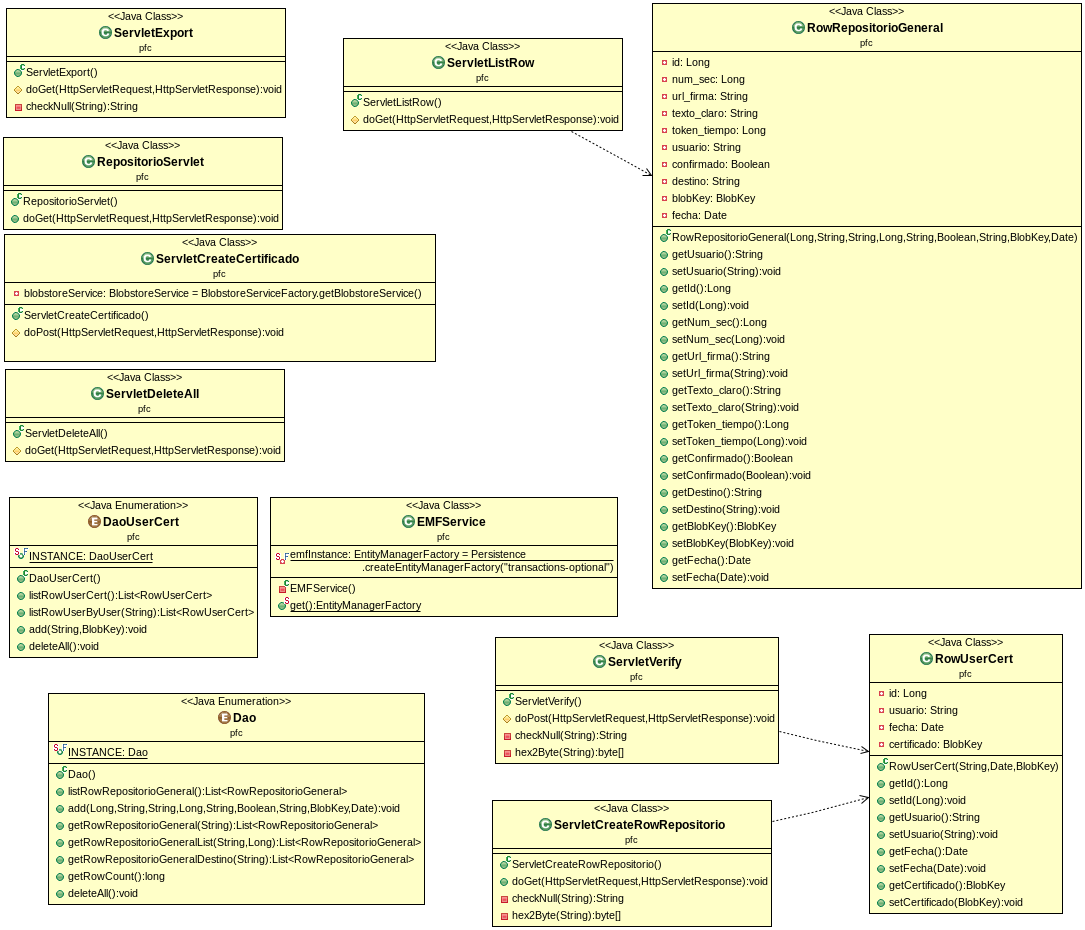
\includegraphics[scale=0.4]{./GoogleAppEngine/imagenes/UML_repositorio.png}
  \caption{Detalles de las clases Repositorio General.}
  \label{fig:clasesReposotorioGeneral}
\end{figure}

\begin{itemize}

\item \textbf{Dao.java:} al igual en el servidor de timestamp esta clase es la encargada de hacer todas operaciones relacionadas con la base de datos.

\item \textbf{DaoUserCert.java:} como hemos implementado dos bases de datos, una para guardar las firmas y otra para guardar los certificados de clave pública que se necesitan, esta clase es la encargada de realizar todas las operaciones en la base de datos donde se guardan los certificados. 

\item \textbf{RowRepositorioGeneral.java:} esta es la clase con la que se crea la tabla en la que se almacenan las firmas de los usuario, tiene los siguientes campos:  

\begin{lstlisting}[style=Java]
@Id
@GeneratedValue(strategy = GenerationType.SEQUENCE) //	 GenerationType.IDENTITY
private Long id;
private Long num_sec;
private String url_firma;
private String texto_claro;
private Long token_tiempo;
private String usuario;
private Boolean confirmado;
private String destino;
private BlobKey blobKey;
private Date fecha;
\end{lstlisting}

Tiene una clave primaría \lstinline{id} que es usada por la base de datos internamente para el almacenado de la información, \lstinline{num_sec} es el número de secuencia dentro la tabla, que va incrementándose automáticamente, \lstinline{url_firma} es la dirección en la que se puede consultar la firma del texto en claro que está en el campo \lstinline{texto_claro}, se guarda el \lstinline{token_tiempo} que es el \lstinline{num_sec} de en la aplicación web servidor de timestamp. La columna \lstinline{usuario} almacena el usuario que ha realizado la firma, y en la columna \lstinline{destino} se guarda a quien va dirigida la firma. En la columna \lstinline{blobkey} se guarda la referencia al certificado de clave pública que estaba en activo cuando se subió la firma a la aplicación web, la columna \lstinline{confirmado} puede valer \lstinline{true} or \lstinline{false} e indica si al subir la firma se pudo verificar, en \lstinline{fecha} está la fecha en la que se almacenó.

\item \textbf{RowUserCert.java:} Esta clase es la encargada de crear la tabla que usamos para guardar los archivos con la clave pública. Los campos que usaremos para almacenarlos serán los que se pueden ver en el siguiente trozo de código.

\begin{lstlisting}[style=Java]
@Id
@GeneratedValue(strategy = GenerationType.SEQUENCE)
private Long id;
private String usuario;
private Date fecha;
private BlobKey certificado;
\end{lstlisting}

Como podemos ver el campo \lstinline{id} será la clave primaria y como hemos explicado será usado por la base de datos internamente para autogestión de las filas, el campo \lstinline{usuario} guardará una cadena con el email de la persona que ha subido ese archivo, el campo \lstinline{fecha} es la fecha en la que se subió el archivo, \lstinline{certificado} es un campo del tipo \lstinline{BlobKey} que es como la ruta al archivo de certificado.

\end{itemize}

Acto seguido vamos a explicar los diferentes servlets que hemos desarrollado para la aplicación web.

\begin{itemize}

\item \textbf{ServletCreateCertificate.java:} Este servlet es el encargado de añadir a la base de datos el certificado de clave pública. Es usado en la pestaña de certificados de la aplicación web y es llamado cuando se pulsa el botón subir certificado. Se puede observar dicho botón en la figura~\ref{fig:pestanhaCertificados}.

\end{itemize}

\begin{figure}[h]
  \centering
    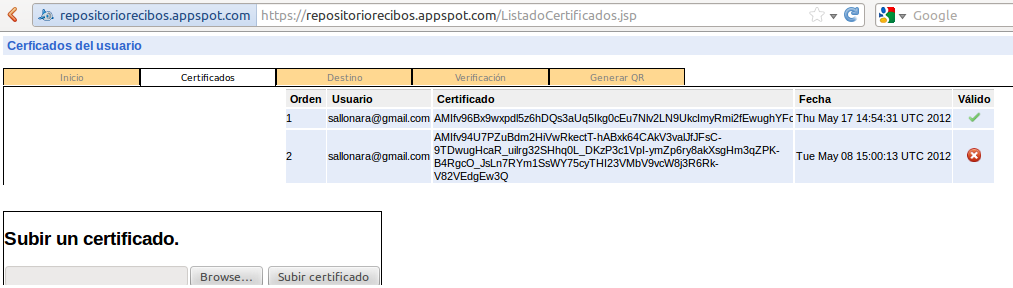
\includegraphics[scale=0.5]{./GoogleAppEngine/imagenes/certificadosRepositorioGeneral.png}
  \caption{Pantallazo de la pestaña certificados.}
  \label{fig:pestanhaCertificados}
\end{figure}

\begin{itemize}

\item \textbf{ServletCreateRowRepositorio.java:} Este servlet está mapeado en la dirección: \url{https://repositoriorecibos.appspot.com/add} y recibe los siguientes parámetros: \url{texto}, \url{url\_firma}, \url{token}, \url{destino} y \url{fecha}. Es el encargado de añadir una fila a la base de datos por cada llamada a dicha dirección, a esta dirección no hay forma de acceder desde la aplicación web. A su vez antes de introducir la fila comprueba que la firma se puede validar y se marca como \lstinline{true} o \lstinline{false} la columna verificado que posteriormente en el archivo \textit{RepositorioGeneralApplication.jsp} se cambiará por una imagen para hacer la verificación más visual. Si hemos podido insertar la fila, el servlet devuelve la cadena ``OK", si no se devuelven varias cadenas con los fallos que han ocurrido.

%\item \textbf{ServletDeleteAll.java:} Servlet ``secreto" que borra todas las filas de firmas almacenadas, hay que llamarlo con un parámetro que es \textit{borrar} con valor \textit{7}

\item \textbf{ServletExport.java:} Este servlet es el encargado de exportar una de las filas para que otra persona pueda comprobar si la firma es válida. Este servlet es llamado cuando se pulsa el botón exportar de la pestaña principal de la aplicación web. Se puede observar en la figura~\ref{fig:botonExportar}

\end{itemize}

\begin{figure}[h]
  \centering
    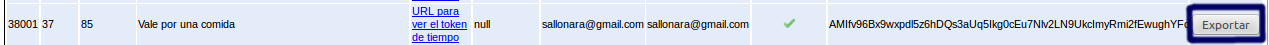
\includegraphics[scale=0.4]{./GoogleAppEngine/imagenes/botonExportar.png}
  \caption{Detalle del botón exportar.}
  \label{fig:botonExportar}
\end{figure}

\begin{itemize}

El servlet recibe los siguiente parámetros:

\begin{lstlisting}[style=Java]
String mensaje = checkNull(req.getParameter("mensaje"));
String url_firma = checkNull(req.getParameter("token"));
String id_blob = checkNull(req.getParameter("id_blob"));
String user = checkNull(req.getParameter("usuario"));
\end{lstlisting}

Una vez se tienen esos parámetros creamos una cadena de texto en la que unimos los siguiente campos y cada parámetro va separado por el separador: ``;/:".

\begin{lstlisting}[style=Java]
String cadACodificar = mensaje + ";/:" + url_firma + ";/:" + id_blob + ";/:" + user;
\end{lstlisting}

Acto seguido codificamos la cadena con \lstinline{Base64}\footnote{Para más información puede consultar: \url{http://en.wikipedia.org/wiki/Base64}}, que es una forma simple de codificar los caracteres para que no viajen en texto claro.

\begin{lstlisting}[style=Java]
String cadCodificada = Base64.encode(cadACodificar.getBytes("UTF-8"));
\end{lstlisting}

También añadimos unos limitadores para que cuando tengamos que decodificar ese mensaje podamos saber donde empiezan y donde termina la exportación.
\begin{lstlisting}[style=Java]
pw.println("BEGIN EXPORT");
pw.println("--------------------------");
pw.println(cadCodificada);
pw.println("--------------------------");
pw.println("END EXPORT");
\end{lstlisting}

\item \textbf{ServletListRow.java:} Este servlet es el encargado en devolver todas las filas de la tabla que pertenecen a un usuario. La forma de hacerlo es la siguiente, primero se identifica el usuario con el que se ha logueado de esta forma:

\begin{lstlisting}[style=Java]
UserService userService = UserServiceFactory.getUserService();
User user = userService.getCurrentUser();
\end{lstlisting}

Una vez se consigue el usuario se llama a la función \lstinline{public List<RowRepositorioGeneral> getRowRepositorioGeneralList(String userId, Long num_sec)} de la clase \lstinline{Dao.java}, esta última función nos devuelve una lista con todas las filas. Al llamar al servlet le pasaremos el último número de secuencia que tenemos guardado en el telefono móvil, para así agilizar las transferencias de datos, de esta forma solo nos devolverá las filas nuevas. La forma de devolvernos las filas será mediante una estructura llamada \lstinline{JSONArray}, que es un objeto que dentro contiene varios objetos \lstinline{JSON}\footnote{Para saber que es un objeto \lstinline{JSON} pueden consultar los siguientes enlaces: \url{http://www.json.org/} o \url{http://en.wikipedia.org/wiki/JSON}}.

La creación de los objetos \lstinline{JSON} la realizamos de la siguiente forma:

\begin{lstlisting}[style=Java]
JSONObject jsonObject = new JSONObject();

jsonObject.put("num_sec", rowRepositorioGeneral.getNum_sec().toString());
jsonObject.put("texto", rowRepositorioGeneral.getTexto_claro());
jsonObject.put("url_firma", rowRepositorioGeneral.getUrl_firma());
jsonObject.put("token_tiempo", rowRepositorioGeneral.getToken_tiempo().toString());
jsonObject.put("usuario",rowRepositorioGeneral.getUsuario());
jsonObject.put("fecha", rowRepositorioGeneral.getFecha().toString());
jsonObject.put("verificado", rowRepositorioGeneral.getConfirmado().toString());
jsonObject.put("destino", rowRepositorioGeneral.getDestino());
\end{lstlisting}

Ese objeto \lstinline{JSON} se añade un objeto \lstinline{JSONArray}, que es el que devolveremos como respuesta final de la ejecución de nuestro servlet y que espera la aplicación Android.

\item \textbf{ServletVerify.java:} Este servlet es el utilizado en la pestaña verificar de nuestra aplicación web, como se puede observar en la figura~\ref{fig:pestanhaVerificar}

\end{itemize}

\begin{figure}[h]
  \centering
    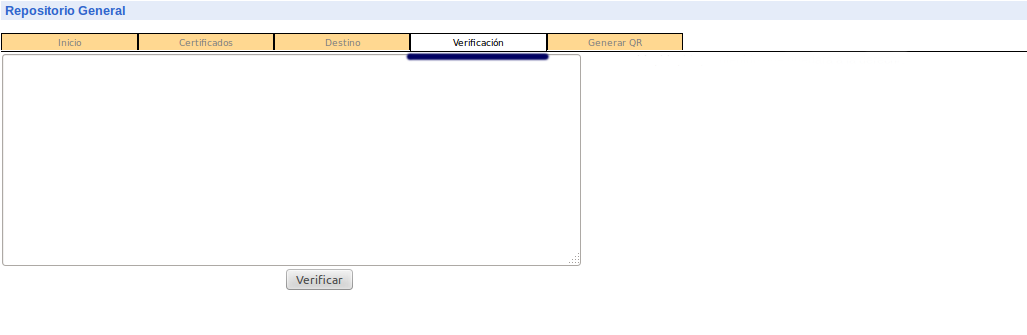
\includegraphics[scale=0.5]{./GoogleAppEngine/imagenes/pestanhaVerificar.png}
  \caption{Detalle de la pestaña verificación.}
  \label{fig:pestanhaVerificar}
\end{figure}

\begin{itemize}

Podemos observar hay un cuadro de texto para introducir la cadena que devuelve el botón exportar. Cualquier usuario puede verificar si una firma es correcta o no. En este servlet se hace el proceso contrario que hicimos en exportar, quitamos los indicadores de inicio y final de exportación, desencriptamos la cadena en \lstinline{Base64} y hacemos varias comprobaciones. Comprobamos que en la fecha en la que se firmó el certificado era válido y que no habíamos revocado dicho certificado, también se comprueba que no fuera reemplazado por otro certificado antes de su expiración, ya que entonces la firma no sería válida. También comprobamos la integridad del mensaje, que la cadena no esté mal formada y que siga el formato que hemos obligado anteriormente.

\end{itemize}

Los archivos JSP que hemos creado en su mayoría solo rellenan tablas dinámicamente haciendo llamadas a funciones de la clase \lstinline{Dao.java}. Solo hay uno que no realiza esas funciones que es el siguiente:

\begin{itemize}

\item \textbf{GenerarQR.jsp:} Este archivo JSP es el que se muestra en la pestaña \textit{Generar QR}, se puede ver en la figura~\ref{fig:pestanhaQR}. Su función es generar un código QR para que pueda ser leído por la aplicación del móvil. Hay que rellenar los campos de destino y el texto que queremos que firme dicha persona. Al darle a \textit{Generar código QR} se hace una llamada a la API Google Chart y se genera un código QR que contiene dichas cadenas y se muestra en la parte de la derecha, como se puede ver en la figura~\ref{fig:codigoQR}.

\end{itemize}

\begin{figure}[h]
  \centering
    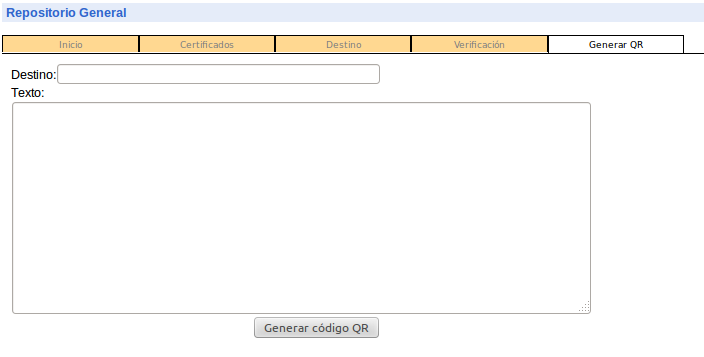
\includegraphics[scale=0.5]{./GoogleAppEngine/imagenes/pestanhaQR.png}
  \caption{Pestaña para generar el código QR.}
  \label{fig:pestanhaQR}
\end{figure}

\begin{figure}[h]
  \centering
    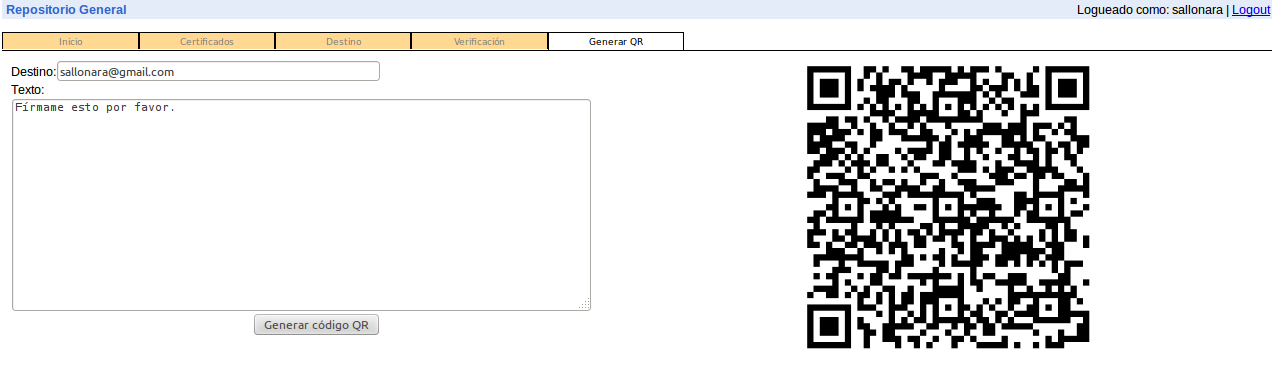
\includegraphics[scale=0.4]{./GoogleAppEngine/imagenes/codigoQR.png}
  \caption{Pestaña con el código QR generado.}
  \label{fig:codigoQR}
\end{figure}




